% !TEX root = ../article.tex

\section{Methodology and specifications}

% !TEX root = ../article.tex

\newcommand{\minimum}{
(x_{min},y_{min}) = {-\pi/2,-\pi/2}
\label{eqn:xymin}
}

\newcommand{\conservationMass}{
\nabla \cdot \vec{u} = 0
\label{eqn:conservationMass}
}

\newcommand{\conservationMomentum}{
\rho (\vec{u} \cdot \nabla) \vec{u} - \mu \nabla^2 \vec{u} = - \nabla P + \vec{F}
\label{eqn:conservationMomentum}
}

\newcommand{\conservationEnergy}{
\rho c_{p} (\vec{u} \cdot \nabla) T - k \nabla^2 T = \gamma \phi
\label{eqn:conservationEnergy}
}

\newcommand{\neutronDiffusion}{
\nabla^2 \phi + B^2 \phi = 0
\label{eqn:neutronDiffusion}
}

\newcommand{\xyParametrization}{
\begin{aligned}
    \alpha(x) &= \frac{\pi}{a} (x - x_{\text{min}}) \\
     \beta(y) &= \frac{\pi}{b} (y - y_{\text{min}})
\end{aligned}
\label{eqn:xyParametrization}
}

\newcommand{\solutionVelocity}{
\begin{aligned}
    u_{x}(x,y) &=  \sin(\alpha)\cos(\beta) \\
    u_{y}(x,y) &= -\cos(\alpha)\sin(\beta)
\end{aligned}
\label{eqn:solutionVelocity}
}

\newcommand{\solutionPressure}{
P(x,y) = P_{\text{c}} + \rho \frac{\cos^2(\alpha) + \cos^2(\beta)}{2}
\label{eqn:solutionPressure}
}

\newcommand{\solutionTemperature}{
T(x,y) = T_{\text{b}} + \Delta T_{\text{c}} \sin(\alpha)\sin(\beta)
\label{eqn:solutionTemperature}
}

\newcommand{\solutionFlux}{
\phi(x,y) = \phi_{\text{c}} \sin(\alpha)\sin(\beta)
\label{eqn:solutionFlux}
}

\newcommand{\momentumForcingTerms}{
\vec{F} = 2 \mu \vec{u}
\label{eqn:momentumForcingTerms}
}

\newcommand{\BCvelocity}{
\begin{aligned}
    &u_{x}(x,-\pi/2) =  \sin(\alpha) \\
    &u_{x}(x,\pi/2)  = -\sin(\alpha) \\
    &u_{y}(-\pi/2,y) = -\sin(\beta)  \\
    &u_{y}(\pi/2,y)  =  \sin(\beta)
\end{aligned}
\label{eqn:BCvelocity}
}

\newcommand{\bucklingGeometrical}{
B_{\text{g}}^2 = \left( \frac{\pi}{a} \right)^2 + \left( \frac{\pi}{b} \right)^2
\label{eqn:bucklingGeometrical}
}

\newcommand{\bucklingMaterial}{
B_{\text{m}}^2 = \frac{\frac{\overline{\nu} \Sigma_{\text{f}}}{k_{\text{eff}}} - \Sigma_{\text{a}}}{D}
\label{eqn:bucklingMaterial}
}

\newcommand{\diffusionCoefficient}{
D = \frac{1}{3(\Sigma_{\text{s}} + \Sigma_{\text{a}})}
\label{eqn:diffusionCoefficient}
}

\newcommand{\deltaT}{
\gamma \phi_{\text{c}} = 2k \Delta T_{\text{c}} \left( \left(\frac{\pi}{a}\right)^{2} + \left(\frac{\pi}{b}\right)^{2} \right) \\
\label{eqn:deltaT}
}

\newcommand{\integralFlux}{
\Phi = \int_{0}^{1} \int_{-\pi/2}^{\pi/2} \int_{-\pi/2}^{\pi/2} \phi_{\text{c}} \sin(\alpha)\sin(\beta) dx dy dz = 4 \phi_{\text{c}}
\label{eqn:integralFlux}
}

\newcommand{\LOneNorm}{
\norm{r - r_{ \text{ref} } }_{1} = \frac{1}{\Omega} \sum_{n=1}^{N} \omega_{n} \abs{ r_{n} - r_{ n,\text{ref} } }
\label{eqn:L1norm}
}

\newcommand{\LTwoNorm}{
\norm{ r - r_{ \text{ref} } }_{2} = \left( \frac{1}{\Omega} \sum_{n=1}^{N} \omega_{n} \abs{ r_{n} - r_{ n,\text{ref} } }^{2} \right) ^{\frac{1}{2}}
\label{eqn:L2norm}
}


\subsection{Equations to solve}

Equations \ref{eqn:conservationMass}, \ref{eqn:conservationMomentum}, and \ref{eqn:conservationEnergy}, collectively known as the Navier-Stokes equations, represent the conservation of mass, momentum and energy for an incompressible flow.

\begin{equation}
    \conservationMass
\end{equation}

\begin{equation}
    \conservationMomentum
\end{equation}

\begin{equation}
    \conservationEnergy
\end{equation}

\nomenclature{$\vec{u}$}{Velocity vector}
\nomenclature{$P$}{Pressure}
\nomenclature{$T$}{Temperature}
\nomenclature{$\phi$}{Neutron flux}

\nomenclature{$\rho$}{Density}
\nomenclature{$\vec{F}$}{Momentum source vector}
\nomenclature{$\mu$}{Dynamic viscosity}
\nomenclature{$c_{p}$}{Specific heat capacity at constant pressure}
\nomenclature{$k$}{Thermal conductivity}
\nomenclature{$\gamma$}{Flux to power conversion factor}

The following equation (\ref{eqn:neutronDiffusion}) is the one-group neutron diffusion equation expressed in terms of the reactor buckling.

\begin{equation}
    \neutronDiffusion
\end{equation}

\nomenclature{$B$}{Buckling}

These 4 equations represent the multiphysics problem that is to be verified by this work.
The usual nomenclature has been used in all equations, but a detailed nomenclature definition can be found at the end of the paper.

In equation \ref{eqn:conservationMomentum} a forcing term $ \vec{F} $ was added on the right-hand side, making the equation a slightly modified version of the usual one.
It is typically hard to satisfy non-trivial analytical solutions in the usual equation, therefore a simple manufactured solution was used.

The method of manufactured solutions for code verification circumvents the need for an analytical solution to satisfy the exact equations, proposing instead the use of a modified equation to satisfy the analytical solution \cite{oberkampf_verification_2010, knupp_verification_2002, roache_verification_1998}.
In order to use this method for code verification, it is necessary that the code allows an arbitrary forcing term to be inserted into the equations.
This capability is present in all standard OpenFOAM solvers as "fvOptions" and has been implemented in the GeN-Foam fluid mechanics solver during this work.
Additional information on how this functionality works can be found in the GeN-Foam test case files at the GitHub repository provided and in OpenFOAM tutorials.

\subsection{Solution domain specification}

The proposed case is a square domain centred at point (0,0), with dimensions of $ \pi $ meters by $ \pi $ meters, as shown in figure \ref{fig:domain}.

\begin{figure}[htbp]
    \centering
    \raisebox{0mm}[65mm][0mm]{
    % !TEX root = ../../article.tex

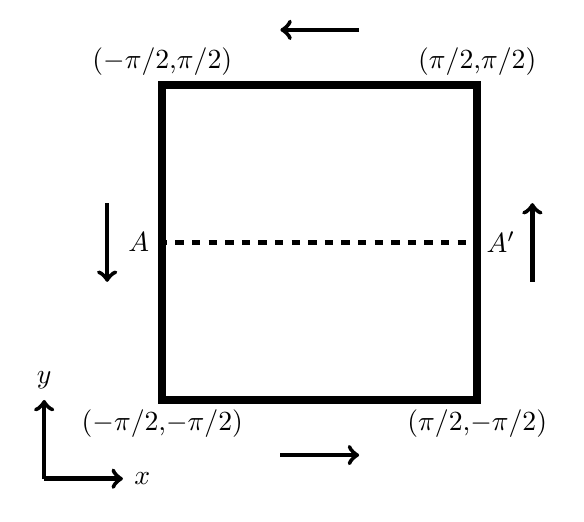
\begin{tikzpicture}
	\draw[line width=1mm] (-2,-2) rectangle (2,2);
    % axes
	\draw[->,ultra thick] (-3.5,-3)--(-2.5,-3) node[right]{$x$};
	\draw[->,ultra thick] (-3.5,-3)--(-3.5,-2) node[above]{$y$};
    % notable points
    \node[] at (-2,-2.3) (bl_corner) {($-\pi/2$,$-\pi/2$)};
    \node[] at (2,-2.3) (br_corner) {($\pi/2$,$-\pi/2$)};
    \node[] at (-2,2.3) (tl_corner) {($-\pi/2$,$\pi/2$)};
    \node[] at (2,2.3) (tr_corner) {($\pi/2$,$\pi/2$)};
	% lines AA' and BB'
	\node[] at (-2.3,0) (a) {$A$};
	\node[] at (2.3,0) (b) {$A'$};
	\draw[dashed,ultra thick] (a.east)--(b);
	% \node[] at (0,-2.3) (c) {$B$};
	% \node[] at (0,2.3) (d) {$B'$};
	% \draw[dashed,ultra thick] (c)--(d);
	% boundary velocity arrows
	\draw[->,ultra thick] (0.5,2.7)--(-0.5,2.7); %top
    \draw[->,ultra thick] (-0.5,-2.7)--(0.5,-2.7); %bottom
    \draw[->,ultra thick] (-2.7,0.5)--(-2.7,-0.5); %left
    \draw[->,ultra thick] (2.7,-0.5)--(2.7,0.5); %right
\end{tikzpicture}

    }
    \caption{Solution domain}
    \label{fig:domain}
\end{figure}

This is a very simple domain, but such simplicity is desirable for verification activities.
It reduces the complexities introduced by the mesh into the verification procedure, and allows systematic refinement of the mesh.

For later reference, it is convenient to define the point at the left-bottom corner of the domain as follows:

\begin{equation}
    \minimum
\end{equation}

Care was taken in selecting a domain that is centered on (0,0) instead of placing the $ (x_{min},y_{min}) $ point at (0,0).
If the second option had been taken, a round-off error would be introduced because the code can compute $\sin(0)$ exactly, but not $\sin(\pi)$.

\subsection{Analytical solutions}

In this section, we present the analytical solutions that we would like to recover from the numerical experiments.
In order to simplify the analytical solutions, to be presented further on, $ \alpha $ and $ \beta $ parameters are defined as follows:

\begin{equation}
    \xyParametrization
\end{equation}

Where $ a $ and $ b $ are the dimensions of the domain on the x and y directions.
Written in this manner, the problem becomes invariant to stretching (variations of $ a $ or $ b $) or translation (variations of $ x_{\text{min}} $ or $ y_{\text{min}} $) in any direction.
For the particular case proposed, $ a = b = \pi \ \text{m} $, resulting in a immediate simplification of equations \ref{eqn:xyParametrization}.

Below, we can see the set of analytical solutions imposed for velocity, pressure, temperature and flux, parametrized by $ \alpha $ and $ \beta $ previously defined.
In equation \ref{eqn:solutionPressure}, $ P_{\text{c}} $ represents the pressure at the centre of the cavity, which is the minimum pressure and also the reference one.
Similarly, $ T_{\text{b}} $ in equation \ref{eqn:solutionTemperature} represents the constant temperature at the boundaries of the domain, which will be specified later on, while $ \Delta T_{\text{c}} $ represents an amplitude above this baseline at the centre, which depends on simulation parameters to be discussed.
Equation \ref{eqn:solutionFlux} is the flux in the domain, and $ \phi_{\text{c}} $ is flux in the centre, or an amplitude above a baseline along which flux is taken as 0.

\begin{equation}
    \solutionVelocity
\end{equation}

\begin{equation}
    \solutionPressure
\end{equation}

\begin{equation}
    \solutionTemperature
\end{equation}

\begin{equation}
    \solutionFlux
\end{equation}

As previously mentioned, the set of equations is arbitrary.
It does not have to be a physical problem in any sense.
The only requirement is for \textbf{solutions to be continuous}.
Another desirable, but not strictly necessary property is for \textbf{solutions to be infinitely differentiable}, avoiding the disappearance of any term in equations \ref{eqn:conservationMass}-\ref{eqn:neutronDiffusion} due to differentiation.

By inserting the analytical solutions \ref{eqn:solutionVelocity} and \ref{eqn:solutionPressure} into equation \ref{eqn:conservationMomentum}, the forcing term $ \vec{F} $ in equation \ref{eqn:conservationMomentum} is derived as:

\begin{equation}
    \momentumForcingTerms
\end{equation}

Equations were purposely chosen to give a very simple arbitrary source, contrary to the usual sources generated by the method of manufactured solutions, containing many terms.
This was recognized as a good initial approach that allowed testing the arbitrary source functionality just implemented, which requires coding in C++ and is a relatively advanced functionality in OpenFOAM.
In addition, it is simple enough to allow derivation by hand, allowing development and verification of a symbolic mathmatics script to derive the usual extensive forcing terms in the future.

\subsection{Boundary conditions}

Evaluating equation \ref{eqn:solutionVelocity} at the domain boundaries, it is possible to specify the velocity boundary conditions as shown in equations \ref{eqn:BCvelocity}.
Each one is a non-uniform Dirichlet boundary condition that is relatively complex to implement in OpenFOAM, requiring the use of the "codedFixedValue" boundary condition.
To better understand how this particular boundary condition is coded, the reader is again referred to the GeN-Foam test case files at the provided GitHub repository.

From the boundary conditions for velocity, it is possible to infer qualitatively that, in this problem, the fluid flows in a counter-clockwise pattern with velocity reducing to 0 at the corners of the domain.

\begin{equation}
    \BCvelocity
\end{equation}

Since the problem is incompressible, the absolute pressure of the system is not important, a reference pressure of $ 10^{5} \ \text{Pa} $ was given since the code requires some value.
What actually matters is the pressure difference created by dynamic forces in the system, commonly known as gauge pressure or, more rigorously, as sealed gauge pressure with the reference pressure as specified.
The appropriate boundary condition for this system sets the gradient of pressure normal to the wall to 0.
This represents an uniform Neumann boundary condition, which also satisfies equation \ref{eqn:solutionPressure}.

For temperature, a uniform Dirichlet boundary condition of $ T_{b} = 1000 \ \text{K} $ was used, which results from evaluating equation \ref{eqn:solutionTemperature} at the boundaries.
This effectively represents an infinite heat sink outside the system with the set temperature.

The neutron flux is set to 0 at the boundaries, also resulting from evaluation of equation \ref{eqn:solutionFlux}.
While this is a quite unusual boundary condition for the neutron diffusion equation, it should be emphasized that the main targets of this verification are the solvers, not the boundary conditions available.
An albedo boundary condition is implemented in GeN-Foam, and could be used, but this should be done only after the neutron diffusion solver is verified.

All the boundary conditions, with the possible exception of the velocity one,  should be readily available in any package for solution of PDEs.
The velocity boundary condition might be a bit more challenging due to its non-uniformity.

\subsection{Parameters}

Table \ref{table:fluidProperties} shows the parameters used for the fluid in this problem.
All the parameters are arbitrary, but their choice requires some consideration.

\begin{table}[htbp]
	\caption{Fluid properties}
	\centering
	% !TEX root = ../../article.tex

\begin{tabular}{l l}
	\toprule

	Parameter & Value  \\

	\midrule

	Density                & 1000 $ \text{kg} \cdot \text{m}^{-3} $ \\
	Specific heat capacity & 1 $ \text{J} \cdot \text{kg}^{-1} \cdot \text{K}^{-1} $ \\
	Thermal conductivity   & 50 $ \text{W} \cdot \text{m}^{-1} \cdot \text{K}^{-1} $ \\
    Dynamic viscosity      & 50 $ \text{Pa} \cdot \text{s} $ \\

	\bottomrule
\end{tabular}

	\label{table:fluidProperties}
\end{table}

Dynamic viscosity is high, compared to physically sensible values, in order to force the flow regime to be laminar despite such a large domain.
In addition, all the parameters in the table are related in choice in order to keep the advective and diffusive terms in the Navier-Stokes equation in balance so that both are similarly exercised.
For example, the choice of specific heat is related to the choice of density and thermal conductivity in order to keep the terms of equation \ref{eqn:conservationEnergy} in balance.
If this balance is not taken into account in and, for example, a high value is given to specific heat while keeping density and thermal conductivity unchanged, numerical noise in the advection term will become significant.
This happens because the advection term of the energy conservation equation is analytically 0, but numerically will be a very small non-zero number (of the order of $ 10^{-8} $).
This very small number (numerical noise) will be multiplied by a very high value ($ \text{density} \cdot \text{specific heat capacity} $) and the term will become significant compared to the diffusion one.
This type of carelessness negatively impacts the solution.

The solution of equation \ref{eqn:neutronDiffusion} requires neutronics parameters, which are also arbitrary to a certain extent.
Equation \ref{eqn:bucklingGeometrical} is the geometrical buckling of a 2D square homogenous unreflected reactor with extrapolation distance 0.
From the equation, and reminding that $ a = b = \pi \ \text {m} $, the problem has $ B_{g}^2 = 2 \ \text{m}^{-2} $.

\begin{equation}
    \bucklingGeometrical
\end{equation}

In order for the reactor to be critical, the material buckling, given by the following equation, has to be equal to the previously calculated geometrical one ($ B_{g}^2 = B_{m}^2 $) \cite{stacey_nuclear_2007}.

\begin{equation}
    \bucklingMaterial
\end{equation}

The neutron diffusion coefficient $ D $ in equation \ref{eqn:bucklingMaterial}, considering isotropic scattering, is given by:

\begin{equation}
    \diffusionCoefficient
\end{equation}

From equations \ref{eqn:bucklingMaterial} and \ref{eqn:diffusionCoefficient}, we generate arbitrary one-group cross-sections considering the following criteria:

\begin{enumerate}
    \item $ k_{\text{eff}} = 1 $
    \item $ D = 2 \cdot 10^{-2} \ \text{m} $
    \item $ \Sigma_{\text{a}} = 1 \ \text{m}^{-1} $
\end{enumerate}

Where item 1 is for convenience, 2 is to work with a diffusion coefficient of the same order of magnitude as the mesh size, and 3 is to have $ \Sigma_{\text{a}} << \Sigma_{\text{s}} $, which is a condition for the diffusion theory to be valid.
The neutronic parameters prescribed by the criteria and the calculated ones are consolidated in table \ref{table:neutronicProperties}.

\begin{table}[htbp]
    \caption{Neutronic properties}
    \centering
    % !TEX root = ../../article.tex

\begin{tabular}{l l}
    \toprule

    Parameter          & Value  \\

    \midrule

    $ D $                                   & $ 2 \cdot 10^{-2} \ \text{m} $ \\
    $ \Sigma_{\text{a}} $                   & 1 $ \text{m}^{-1} $ \\
    $ \Sigma_{\text{s}} $                   & 15.666\dots $ \text{m}^{-1} $ \\
    $ \overline{\nu} \Sigma_{\text{f}} $    & 1.04 $ \text{m}^{-1} $ \\
    $ \gamma $                              & 1 $ \text{J}\cdot \text{m}^{-1} $ \\

    \bottomrule
\end{tabular}

    \label{table:neutronicProperties}
\end{table}

Inserting the analytical solutions \ref{eqn:solutionVelocity}, \ref{eqn:solutionTemperature}, and \ref{eqn:solutionFlux} into equation \ref{eqn:conservationEnergy}, we get:

\begin{equation}
    \deltaT
\end{equation}

For a flux to power conversion ratio (commonly known as kappa-fission) $ \gamma = 1 \ \text{J}\cdot \text{m}^{-1} $, $ k = 50 \ \text{W} \cdot \text{m}^{-1} \cdot \text{K}^{-1} $ and an arbitrary $ \Delta T_{\text{c}} = 100 \ \text{K} $, we get a $ \phi_{\text{c}} = 10^{4} \ \text{m}^{-2} \cdot \text{s}^{-1} $.
Usually, codes normalize the flux according to reactor power, as is the case of GeN-Foam.
To calculate the required power, first it is necessary to integrate the flux $ \phi(x,y) $ given by equation \ref{eqn:solutionFlux} over the domain, getting the integral flux $ \Phi $.
It is important to mention that although the domain is conceptually 2D, all parameter were given with 3D units for better understanding.
However, this implies that in order to achieve strict unit matching the integration has to cover 3 dimensions, where the third dimension over a pseudo-axis z measures $ 1 \ \text {m} $, being numerically irrelevant.

\begin{equation}
    \integralFlux
\end{equation}

If $ \phi_{\text{c}} = 10^{4} \ \text{m}^{-2} \cdot \text{s}^{-1} $, as previously mentioned, then $ \Phi = 4 \cdot 10^{4} \ \text{m} \cdot \text{s}^{-1} $ .
Considering $ \gamma = 1 \ \text{J}\cdot \text{m}^{-1} $ once again, power will be equal to $ \gamma \Phi = 4 \cdot 10^{4} \ \text{W} $.
